% Options for packages loaded elsewhere
\PassOptionsToPackage{unicode}{hyperref}
\PassOptionsToPackage{hyphens}{url}
%
\documentclass[
]{article}
\usepackage{lmodern}
\usepackage{amssymb,amsmath}
\usepackage{ifxetex,ifluatex}
\ifnum 0\ifxetex 1\fi\ifluatex 1\fi=0 % if pdftex
  \usepackage[T1]{fontenc}
  \usepackage[utf8]{inputenc}
  \usepackage{textcomp} % provide euro and other symbols
\else % if luatex or xetex
  \usepackage{unicode-math}
  \defaultfontfeatures{Scale=MatchLowercase}
  \defaultfontfeatures[\rmfamily]{Ligatures=TeX,Scale=1}
\fi
% Use upquote if available, for straight quotes in verbatim environments
\IfFileExists{upquote.sty}{\usepackage{upquote}}{}
\IfFileExists{microtype.sty}{% use microtype if available
  \usepackage[]{microtype}
  \UseMicrotypeSet[protrusion]{basicmath} % disable protrusion for tt fonts
}{}
\makeatletter
\@ifundefined{KOMAClassName}{% if non-KOMA class
  \IfFileExists{parskip.sty}{%
    \usepackage{parskip}
  }{% else
    \setlength{\parindent}{0pt}
    \setlength{\parskip}{6pt plus 2pt minus 1pt}}
}{% if KOMA class
  \KOMAoptions{parskip=half}}
\makeatother
\usepackage{xcolor}
\IfFileExists{xurl.sty}{\usepackage{xurl}}{} % add URL line breaks if available
\IfFileExists{bookmark.sty}{\usepackage{bookmark}}{\usepackage{hyperref}}
\hypersetup{
  pdftitle={King Sejong's National Referendum on Tax Reform},
  pdfauthor={coop711},
  hidelinks,
  pdfcreator={LaTeX via pandoc}}
\urlstyle{same} % disable monospaced font for URLs
\usepackage[margin=1in]{geometry}
\usepackage{color}
\usepackage{fancyvrb}
\newcommand{\VerbBar}{|}
\newcommand{\VERB}{\Verb[commandchars=\\\{\}]}
\DefineVerbatimEnvironment{Highlighting}{Verbatim}{commandchars=\\\{\}}
% Add ',fontsize=\small' for more characters per line
\usepackage{framed}
\definecolor{shadecolor}{RGB}{248,248,248}
\newenvironment{Shaded}{\begin{snugshade}}{\end{snugshade}}
\newcommand{\AlertTok}[1]{\textcolor[rgb]{0.94,0.16,0.16}{#1}}
\newcommand{\AnnotationTok}[1]{\textcolor[rgb]{0.56,0.35,0.01}{\textbf{\textit{#1}}}}
\newcommand{\AttributeTok}[1]{\textcolor[rgb]{0.77,0.63,0.00}{#1}}
\newcommand{\BaseNTok}[1]{\textcolor[rgb]{0.00,0.00,0.81}{#1}}
\newcommand{\BuiltInTok}[1]{#1}
\newcommand{\CharTok}[1]{\textcolor[rgb]{0.31,0.60,0.02}{#1}}
\newcommand{\CommentTok}[1]{\textcolor[rgb]{0.56,0.35,0.01}{\textit{#1}}}
\newcommand{\CommentVarTok}[1]{\textcolor[rgb]{0.56,0.35,0.01}{\textbf{\textit{#1}}}}
\newcommand{\ConstantTok}[1]{\textcolor[rgb]{0.00,0.00,0.00}{#1}}
\newcommand{\ControlFlowTok}[1]{\textcolor[rgb]{0.13,0.29,0.53}{\textbf{#1}}}
\newcommand{\DataTypeTok}[1]{\textcolor[rgb]{0.13,0.29,0.53}{#1}}
\newcommand{\DecValTok}[1]{\textcolor[rgb]{0.00,0.00,0.81}{#1}}
\newcommand{\DocumentationTok}[1]{\textcolor[rgb]{0.56,0.35,0.01}{\textbf{\textit{#1}}}}
\newcommand{\ErrorTok}[1]{\textcolor[rgb]{0.64,0.00,0.00}{\textbf{#1}}}
\newcommand{\ExtensionTok}[1]{#1}
\newcommand{\FloatTok}[1]{\textcolor[rgb]{0.00,0.00,0.81}{#1}}
\newcommand{\FunctionTok}[1]{\textcolor[rgb]{0.00,0.00,0.00}{#1}}
\newcommand{\ImportTok}[1]{#1}
\newcommand{\InformationTok}[1]{\textcolor[rgb]{0.56,0.35,0.01}{\textbf{\textit{#1}}}}
\newcommand{\KeywordTok}[1]{\textcolor[rgb]{0.13,0.29,0.53}{\textbf{#1}}}
\newcommand{\NormalTok}[1]{#1}
\newcommand{\OperatorTok}[1]{\textcolor[rgb]{0.81,0.36,0.00}{\textbf{#1}}}
\newcommand{\OtherTok}[1]{\textcolor[rgb]{0.56,0.35,0.01}{#1}}
\newcommand{\PreprocessorTok}[1]{\textcolor[rgb]{0.56,0.35,0.01}{\textit{#1}}}
\newcommand{\RegionMarkerTok}[1]{#1}
\newcommand{\SpecialCharTok}[1]{\textcolor[rgb]{0.00,0.00,0.00}{#1}}
\newcommand{\SpecialStringTok}[1]{\textcolor[rgb]{0.31,0.60,0.02}{#1}}
\newcommand{\StringTok}[1]{\textcolor[rgb]{0.31,0.60,0.02}{#1}}
\newcommand{\VariableTok}[1]{\textcolor[rgb]{0.00,0.00,0.00}{#1}}
\newcommand{\VerbatimStringTok}[1]{\textcolor[rgb]{0.31,0.60,0.02}{#1}}
\newcommand{\WarningTok}[1]{\textcolor[rgb]{0.56,0.35,0.01}{\textbf{\textit{#1}}}}
\usepackage{longtable,booktabs}
% Correct order of tables after \paragraph or \subparagraph
\usepackage{etoolbox}
\makeatletter
\patchcmd\longtable{\par}{\if@noskipsec\mbox{}\fi\par}{}{}
\makeatother
% Allow footnotes in longtable head/foot
\IfFileExists{footnotehyper.sty}{\usepackage{footnotehyper}}{\usepackage{footnote}}
\makesavenoteenv{longtable}
\usepackage{graphicx}
\makeatletter
\def\maxwidth{\ifdim\Gin@nat@width>\linewidth\linewidth\else\Gin@nat@width\fi}
\def\maxheight{\ifdim\Gin@nat@height>\textheight\textheight\else\Gin@nat@height\fi}
\makeatother
% Scale images if necessary, so that they will not overflow the page
% margins by default, and it is still possible to overwrite the defaults
% using explicit options in \includegraphics[width, height, ...]{}
\setkeys{Gin}{width=\maxwidth,height=\maxheight,keepaspectratio}
% Set default figure placement to htbp
\makeatletter
\def\fps@figure{htbp}
\makeatother
\setlength{\emergencystretch}{3em} % prevent overfull lines
\providecommand{\tightlist}{%
  \setlength{\itemsep}{0pt}\setlength{\parskip}{0pt}}
\setcounter{secnumdepth}{-\maxdimen} % remove section numbering

\title{King Sejong's National Referendum on Tax Reform}
\author{coop711}
\date{2020-05-18}

\begin{document}
\maketitle

\hypertarget{data}{%
\subsection{Data}\label{data}}

\hypertarget{reading-data}{%
\subsubsection{Reading Data}\label{reading-data}}

Original data came from intenet version of Sejong silok, summarized by
Oh, Ki-Soo.

\begin{Shaded}
\begin{Highlighting}[]
\NormalTok{knitr}\OperatorTok{::}\KeywordTok{include\_graphics}\NormalTok{(}\StringTok{"../pics/sejong\_poll\_data.png"}\NormalTok{)}
\end{Highlighting}
\end{Shaded}

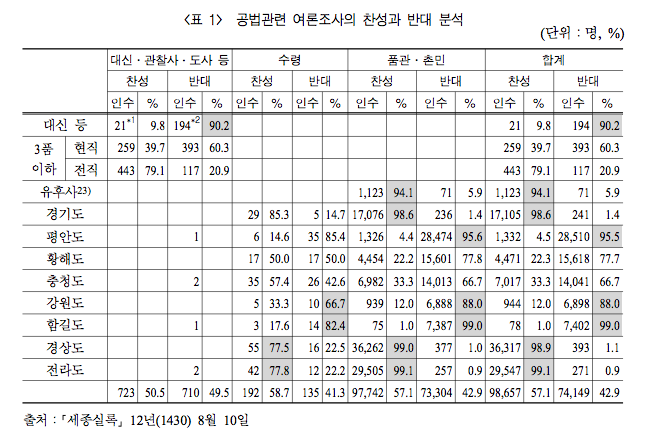
\includegraphics[width=1\linewidth]{../pics/sejong_poll_data}

\begin{Shaded}
\begin{Highlighting}[]
\NormalTok{sejong\_poll \textless{}{-}}\StringTok{ }\KeywordTok{read.table}\NormalTok{(}\StringTok{"../data/sejong\_poll.txt"}\NormalTok{, }\DataTypeTok{header =} \OtherTok{TRUE}\NormalTok{, }\DataTypeTok{stringsAsFactors =} \OtherTok{FALSE}\NormalTok{)}
\KeywordTok{str}\NormalTok{(sejong\_poll)}
\end{Highlighting}
\end{Shaded}

\begin{verbatim}
## 'data.frame':    44 obs. of  4 variables:
##  $ counts: int  21 194 259 393 443 117 1123 71 29 5 ...
##  $ vote  : chr  "yes" "no" "yes" "no" ...
##  $ class : chr  "high" "high" "third.current" "third.current" ...
##  $ region: chr  "Seoul" "Seoul" "Seoul" "Seoul" ...
\end{verbatim}

\begin{Shaded}
\begin{Highlighting}[]
\CommentTok{\# pander(sejong\_poll)}
\KeywordTok{kable}\NormalTok{(sejong\_poll[}\DecValTok{4}\OperatorTok{:}\DecValTok{1}\NormalTok{])}
\end{Highlighting}
\end{Shaded}

\begin{longtable}[]{@{}lllr@{}}
\toprule
region & class & vote & counts\tabularnewline
\midrule
\endhead
Seoul & high & yes & 21\tabularnewline
Seoul & high & no & 194\tabularnewline
Seoul & third.current & yes & 259\tabularnewline
Seoul & third.current & no & 393\tabularnewline
Seoul & third.ex & yes & 443\tabularnewline
Seoul & third.ex & no & 117\tabularnewline
yuhu & ordinary & yes & 1123\tabularnewline
yuhu & ordinary & no & 71\tabularnewline
gyunggi & chief & yes & 29\tabularnewline
gyunggi & chief & no & 5\tabularnewline
gyunggi & ordinary & yes & 17076\tabularnewline
gyunggi & ordinary & no & 236\tabularnewline
pyungan & high & no & 1\tabularnewline
pyungan & chief & yes & 6\tabularnewline
pyungan & chief & no & 35\tabularnewline
pyungan & ordinary & yes & 1326\tabularnewline
pyungan & ordinary & no & 28474\tabularnewline
hwanghae & chief & yes & 17\tabularnewline
hwanghae & chief & no & 17\tabularnewline
hwanghae & ordinary & yes & 4454\tabularnewline
hwanghae & ordinary & no & 15601\tabularnewline
chungcheong & high & no & 2\tabularnewline
chungcheong & chief & yes & 35\tabularnewline
chungcheong & chief & no & 26\tabularnewline
chungcheong & ordinary & yes & 6982\tabularnewline
chungcheong & ordinary & no & 14013\tabularnewline
kangwon & chief & yes & 5\tabularnewline
kangwon & chief & no & 10\tabularnewline
kangwon & ordinary & yes & 939\tabularnewline
kangwon & ordinary & no & 6888\tabularnewline
hamgil & high & no & 1\tabularnewline
hamgil & chief & yes & 3\tabularnewline
hamgil & chief & no & 14\tabularnewline
hamgil & ordinary & yes & 75\tabularnewline
hamgil & ordinary & no & 7387\tabularnewline
gyungsang & chief & yes & 55\tabularnewline
gyungsang & chief & no & 16\tabularnewline
gyungsang & ordinary & yes & 36262\tabularnewline
gyungsang & ordinary & no & 377\tabularnewline
jeolla & high & no & 2\tabularnewline
jeolla & chief & yes & 42\tabularnewline
jeolla & chief & no & 12\tabularnewline
jeolla & ordinary & yes & 29505\tabularnewline
jeolla & ordinary & no & 257\tabularnewline
\bottomrule
\end{longtable}

\hypertarget{factor-conversion}{%
\subsubsection{Factor conversion}\label{factor-conversion}}

We need vote, class, region as \texttt{factor}s. If you leave them as
\texttt{chr}, it will be coerced to factor when you tabulate it
according to alphabetical order, which is not what you want. So, use
\texttt{factor()} to convert them. First, make a working copy vesion of
\texttt{sejong\_poll}

\begin{Shaded}
\begin{Highlighting}[]
\NormalTok{sejong\_poll\_}\DecValTok{2}\NormalTok{ \textless{}{-}}\StringTok{ }\NormalTok{sejong\_poll}
\end{Highlighting}
\end{Shaded}

\begin{Shaded}
\begin{Highlighting}[]
\NormalTok{sejong\_poll\_}\DecValTok{2}\OperatorTok{$}\NormalTok{vote \textless{}{-}}\StringTok{ }\KeywordTok{factor}\NormalTok{(sejong\_poll\_}\DecValTok{2}\OperatorTok{$}\NormalTok{vote, }\DataTypeTok{levels =} \KeywordTok{c}\NormalTok{(}\StringTok{"yes"}\NormalTok{,}\StringTok{"no"}\NormalTok{), }\DataTypeTok{labels =} \KeywordTok{c}\NormalTok{(}\StringTok{"Yes"}\NormalTok{, }\StringTok{"No"}\NormalTok{))}
\end{Highlighting}
\end{Shaded}

You can check that \texttt{labels\ =} is not necessary if same as
levels. Continue with class and region\_

\begin{Shaded}
\begin{Highlighting}[]
\NormalTok{class\_levels \textless{}{-}}\StringTok{ }\KeywordTok{c}\NormalTok{(}\StringTok{"high"}\NormalTok{,}\StringTok{"third.current"}\NormalTok{, }\StringTok{"third.ex"}\NormalTok{, }\StringTok{"chief"}\NormalTok{, }\StringTok{"ordinary"}\NormalTok{)}
\NormalTok{class\_labels \textless{}{-}}\StringTok{ }\KeywordTok{c}\NormalTok{(}\StringTok{"High"}\NormalTok{,}\StringTok{"3rd\_current"}\NormalTok{, }\StringTok{"3rd\_former"}\NormalTok{, }\StringTok{"Chief"}\NormalTok{, }\StringTok{"Commons"}\NormalTok{)}
\NormalTok{sejong\_poll\_}\DecValTok{2}\OperatorTok{$}\NormalTok{class \textless{}{-}}\StringTok{ }\KeywordTok{factor}\NormalTok{(sejong\_poll\_}\DecValTok{2}\OperatorTok{$}\NormalTok{class, }\DataTypeTok{levels =}\NormalTok{ class\_levels, }\DataTypeTok{labels =}\NormalTok{ class\_labels)}
\end{Highlighting}
\end{Shaded}

\begin{Shaded}
\begin{Highlighting}[]
\NormalTok{region\_levels \textless{}{-}}\StringTok{ }\KeywordTok{c}\NormalTok{(}\StringTok{"Seoul"}\NormalTok{,}\StringTok{"yuhu"}\NormalTok{, }\StringTok{"gyunggi"}\NormalTok{, }\StringTok{"pyungan"}\NormalTok{, }\StringTok{"hwanghae"}\NormalTok{, }\StringTok{"chungcheong"}\NormalTok{, }\StringTok{"kangwon"}\NormalTok{, }\StringTok{"hamgil"}\NormalTok{, }\StringTok{"gyungsang"}\NormalTok{, }\StringTok{"jeolla"}\NormalTok{)}
\CommentTok{\# region\_labels \textless{}{-} c("Seoul","Yuhu", "Gyunggi", "Pyungan", "Hwanghae", "Chungcheong", "Kangwon", "Hamgil", "Gyungsang", "Jeolla")}
\NormalTok{region\_labels \textless{}{-}}\StringTok{ }\KeywordTok{c}\NormalTok{(}\StringTok{"SL"}\NormalTok{,}\StringTok{"YH"}\NormalTok{, }\StringTok{"GG"}\NormalTok{, }\StringTok{"PA"}\NormalTok{, }\StringTok{"HH"}\NormalTok{, }\StringTok{"CC"}\NormalTok{, }\StringTok{"KW"}\NormalTok{, }\StringTok{"HG"}\NormalTok{, }\StringTok{"GS"}\NormalTok{, }\StringTok{"JL"}\NormalTok{)}
\NormalTok{sejong\_poll\_}\DecValTok{2}\OperatorTok{$}\NormalTok{region \textless{}{-}}\StringTok{ }\KeywordTok{factor}\NormalTok{(sejong\_poll\_}\DecValTok{2}\OperatorTok{$}\NormalTok{region, }\DataTypeTok{levels =}\NormalTok{ region\_levels, }\DataTypeTok{labels =}\NormalTok{ region\_labels)}
\end{Highlighting}
\end{Shaded}

\begin{Shaded}
\begin{Highlighting}[]
\KeywordTok{str}\NormalTok{(sejong\_poll\_}\DecValTok{2}\NormalTok{)}
\end{Highlighting}
\end{Shaded}

\begin{verbatim}
## 'data.frame':    44 obs. of  4 variables:
##  $ counts: int  21 194 259 393 443 117 1123 71 29 5 ...
##  $ vote  : Factor w/ 2 levels "Yes","No": 1 2 1 2 1 2 1 2 1 2 ...
##  $ class : Factor w/ 5 levels "High","3rd_current",..: 1 1 2 2 3 3 5 5 4 4 ...
##  $ region: Factor w/ 10 levels "SL","YH","GG",..: 1 1 1 1 1 1 2 2 3 3 ...
\end{verbatim}

\begin{Shaded}
\begin{Highlighting}[]
\KeywordTok{kable}\NormalTok{(sejong\_poll\_}\DecValTok{2}\NormalTok{[}\DecValTok{4}\OperatorTok{:}\DecValTok{1}\NormalTok{])}
\end{Highlighting}
\end{Shaded}

\begin{longtable}[]{@{}lllr@{}}
\toprule
region & class & vote & counts\tabularnewline
\midrule
\endhead
SL & High & Yes & 21\tabularnewline
SL & High & No & 194\tabularnewline
SL & 3rd\_current & Yes & 259\tabularnewline
SL & 3rd\_current & No & 393\tabularnewline
SL & 3rd\_former & Yes & 443\tabularnewline
SL & 3rd\_former & No & 117\tabularnewline
YH & Commons & Yes & 1123\tabularnewline
YH & Commons & No & 71\tabularnewline
GG & Chief & Yes & 29\tabularnewline
GG & Chief & No & 5\tabularnewline
GG & Commons & Yes & 17076\tabularnewline
GG & Commons & No & 236\tabularnewline
PA & High & No & 1\tabularnewline
PA & Chief & Yes & 6\tabularnewline
PA & Chief & No & 35\tabularnewline
PA & Commons & Yes & 1326\tabularnewline
PA & Commons & No & 28474\tabularnewline
HH & Chief & Yes & 17\tabularnewline
HH & Chief & No & 17\tabularnewline
HH & Commons & Yes & 4454\tabularnewline
HH & Commons & No & 15601\tabularnewline
CC & High & No & 2\tabularnewline
CC & Chief & Yes & 35\tabularnewline
CC & Chief & No & 26\tabularnewline
CC & Commons & Yes & 6982\tabularnewline
CC & Commons & No & 14013\tabularnewline
KW & Chief & Yes & 5\tabularnewline
KW & Chief & No & 10\tabularnewline
KW & Commons & Yes & 939\tabularnewline
KW & Commons & No & 6888\tabularnewline
HG & High & No & 1\tabularnewline
HG & Chief & Yes & 3\tabularnewline
HG & Chief & No & 14\tabularnewline
HG & Commons & Yes & 75\tabularnewline
HG & Commons & No & 7387\tabularnewline
GS & Chief & Yes & 55\tabularnewline
GS & Chief & No & 16\tabularnewline
GS & Commons & Yes & 36262\tabularnewline
GS & Commons & No & 377\tabularnewline
JL & High & No & 2\tabularnewline
JL & Chief & Yes & 42\tabularnewline
JL & Chief & No & 12\tabularnewline
JL & Commons & Yes & 29505\tabularnewline
JL & Commons & No & 257\tabularnewline
\bottomrule
\end{longtable}

\hypertarget{array}{%
\subsubsection{Array}\label{array}}

We can set up the data as an array

\begin{Shaded}
\begin{Highlighting}[]
\NormalTok{sejong\_poll\_array \textless{}{-}}\StringTok{ }\KeywordTok{xtabs}\NormalTok{(counts }\OperatorTok{\textasciitilde{}}\StringTok{ }\NormalTok{vote }\OperatorTok{+}\StringTok{ }\NormalTok{class }\OperatorTok{+}\StringTok{ }\NormalTok{region, }
                           \DataTypeTok{data =}\NormalTok{ sejong\_poll\_}\DecValTok{2}\NormalTok{)}
\KeywordTok{str}\NormalTok{(sejong\_poll\_array)}
\end{Highlighting}
\end{Shaded}

\begin{verbatim}
##  'xtabs' int [1:2, 1:5, 1:10] 21 194 259 393 443 117 0 0 0 0 ...
##  - attr(*, "dimnames")=List of 3
##   ..$ vote  : chr [1:2] "Yes" "No"
##   ..$ class : chr [1:5] "High" "3rd_current" "3rd_former" "Chief" ...
##   ..$ region: chr [1:10] "SL" "YH" "GG" "PA" ...
##  - attr(*, "call")= language xtabs(formula = counts ~ vote + class + region, data = sejong_poll_2)
\end{verbatim}

\begin{Shaded}
\begin{Highlighting}[]
\NormalTok{sejong\_poll\_array}
\end{Highlighting}
\end{Shaded}

\begin{verbatim}
## , , region = SL
## 
##      class
## vote   High 3rd_current 3rd_former Chief Commons
##   Yes    21         259        443     0       0
##   No    194         393        117     0       0
## 
## , , region = YH
## 
##      class
## vote   High 3rd_current 3rd_former Chief Commons
##   Yes     0           0          0     0    1123
##   No      0           0          0     0      71
## 
## , , region = GG
## 
##      class
## vote   High 3rd_current 3rd_former Chief Commons
##   Yes     0           0          0    29   17076
##   No      0           0          0     5     236
## 
## , , region = PA
## 
##      class
## vote   High 3rd_current 3rd_former Chief Commons
##   Yes     0           0          0     6    1326
##   No      1           0          0    35   28474
## 
## , , region = HH
## 
##      class
## vote   High 3rd_current 3rd_former Chief Commons
##   Yes     0           0          0    17    4454
##   No      0           0          0    17   15601
## 
## , , region = CC
## 
##      class
## vote   High 3rd_current 3rd_former Chief Commons
##   Yes     0           0          0    35    6982
##   No      2           0          0    26   14013
## 
## , , region = KW
## 
##      class
## vote   High 3rd_current 3rd_former Chief Commons
##   Yes     0           0          0     5     939
##   No      0           0          0    10    6888
## 
## , , region = HG
## 
##      class
## vote   High 3rd_current 3rd_former Chief Commons
##   Yes     0           0          0     3      75
##   No      1           0          0    14    7387
## 
## , , region = GS
## 
##      class
## vote   High 3rd_current 3rd_former Chief Commons
##   Yes     0           0          0    55   36262
##   No      0           0          0    16     377
## 
## , , region = JL
## 
##      class
## vote   High 3rd_current 3rd_former Chief Commons
##   Yes     0           0          0    42   29505
##   No      2           0          0    12     257
\end{verbatim}

\hypertarget{votes}{%
\subsection{Votes}\label{votes}}

\hypertarget{total}{%
\subsubsection{Total}\label{total}}

Check the total vote with xtabs()

\begin{Shaded}
\begin{Highlighting}[]
\NormalTok{vote\_total \textless{}{-}}\StringTok{ }\KeywordTok{xtabs}\NormalTok{(counts }\OperatorTok{\textasciitilde{}}\StringTok{ }\NormalTok{vote, }
                    \DataTypeTok{data =}\NormalTok{ sejong\_poll\_}\DecValTok{2}\NormalTok{)}
\KeywordTok{kable}\NormalTok{(}\KeywordTok{t}\NormalTok{(}\KeywordTok{as.matrix}\NormalTok{(vote\_total)), }
      \DataTypeTok{caption =} \StringTok{"Total"}\NormalTok{)}
\end{Highlighting}
\end{Shaded}

\begin{longtable}[]{@{}rr@{}}
\caption{Total}\tabularnewline
\toprule
Yes & No\tabularnewline
\midrule
\endfirsthead
\toprule
Yes & No\tabularnewline
\midrule
\endhead
98657 & 74149\tabularnewline
\bottomrule
\end{longtable}

\begin{Shaded}
\begin{Highlighting}[]
\CommentTok{\# format(prop.table(vote\_total)*100, digits = 3, nsmall = 1)}
\KeywordTok{kable}\NormalTok{(}\KeywordTok{t}\NormalTok{(}\KeywordTok{as.matrix}\NormalTok{(}\KeywordTok{format}\NormalTok{(}\KeywordTok{prop.table}\NormalTok{(vote\_total) }\OperatorTok{*}\StringTok{ }\DecValTok{100}\NormalTok{, }
                         \DataTypeTok{digits =} \DecValTok{3}\NormalTok{, }
                         \DataTypeTok{nsmall =} \DecValTok{1}\NormalTok{))), }
      \DataTypeTok{caption =} \StringTok{"Percentage"}\NormalTok{, }
      \DataTypeTok{align =} \KeywordTok{rep}\NormalTok{(}\StringTok{"r"}\NormalTok{, }\DecValTok{2}\NormalTok{))}
\end{Highlighting}
\end{Shaded}

\begin{longtable}[]{@{}rr@{}}
\caption{Percentage}\tabularnewline
\toprule
Yes & No\tabularnewline
\midrule
\endfirsthead
\toprule
Yes & No\tabularnewline
\midrule
\endhead
57.1 & 42.9\tabularnewline
\bottomrule
\end{longtable}

\begin{Shaded}
\begin{Highlighting}[]
\NormalTok{vote\_total}\FloatTok{.2}\NormalTok{ \textless{}{-}}\StringTok{ }\KeywordTok{apply}\NormalTok{(sejong\_poll\_array, }\DecValTok{1}\NormalTok{, sum)}
\CommentTok{\# kable(t(as.matrix(vote\_total.2)))}
\KeywordTok{kable}\NormalTok{(}\KeywordTok{t}\NormalTok{(}\KeywordTok{as.matrix}\NormalTok{(vote\_total}\FloatTok{.2}\NormalTok{)), }
      \DataTypeTok{caption =} \StringTok{"Total"}\NormalTok{)}
\end{Highlighting}
\end{Shaded}

\begin{longtable}[]{@{}rr@{}}
\caption{Total}\tabularnewline
\toprule
Yes & No\tabularnewline
\midrule
\endfirsthead
\toprule
Yes & No\tabularnewline
\midrule
\endhead
98657 & 74149\tabularnewline
\bottomrule
\end{longtable}

\hypertarget{vote-by-class}{%
\subsubsection{Vote by class}\label{vote-by-class}}

\begin{Shaded}
\begin{Highlighting}[]
\NormalTok{vote\_class \textless{}{-}}\StringTok{ }\KeywordTok{xtabs}\NormalTok{(counts }\OperatorTok{\textasciitilde{}}\StringTok{ }\NormalTok{vote }\OperatorTok{+}\StringTok{ }\NormalTok{class, }
                    \DataTypeTok{data =}\NormalTok{ sejong\_poll\_}\DecValTok{2}\NormalTok{)}
\KeywordTok{kable}\NormalTok{(vote\_class, }
      \DataTypeTok{caption =} \StringTok{"By Class"}\NormalTok{)}
\end{Highlighting}
\end{Shaded}

\begin{longtable}[]{@{}lrrrrr@{}}
\caption{By Class}\tabularnewline
\toprule
& High & 3rd\_current & 3rd\_former & Chief & Commons\tabularnewline
\midrule
\endfirsthead
\toprule
& High & 3rd\_current & 3rd\_former & Chief & Commons\tabularnewline
\midrule
\endhead
Yes & 21 & 259 & 443 & 192 & 97742\tabularnewline
No & 200 & 393 & 117 & 135 & 73304\tabularnewline
\bottomrule
\end{longtable}

\begin{Shaded}
\begin{Highlighting}[]
\NormalTok{vote\_class\_a \textless{}{-}}\StringTok{ }\KeywordTok{apply}\NormalTok{(sejong\_poll\_array, }\DecValTok{1}\OperatorTok{:}\DecValTok{2}\NormalTok{, sum)}
\KeywordTok{kable}\NormalTok{(vote\_class\_a, }
      \DataTypeTok{caption =} \StringTok{"By Class"}\NormalTok{)}
\end{Highlighting}
\end{Shaded}

\begin{longtable}[]{@{}lrrrrr@{}}
\caption{By Class}\tabularnewline
\toprule
& High & 3rd\_current & 3rd\_former & Chief & Commons\tabularnewline
\midrule
\endfirsthead
\toprule
& High & 3rd\_current & 3rd\_former & Chief & Commons\tabularnewline
\midrule
\endhead
Yes & 21 & 259 & 443 & 192 & 97742\tabularnewline
No & 200 & 393 & 117 & 135 & 73304\tabularnewline
\bottomrule
\end{longtable}

\hypertarget{commons-vs-bureaucrats}{%
\subsubsection{Commons vs Bureaucrats}\label{commons-vs-bureaucrats}}

We need to analyse Commons separately.

\begin{Shaded}
\begin{Highlighting}[]
\NormalTok{sejong\_poll\_}\DecValTok{2}\OperatorTok{$}\NormalTok{class\_}\DecValTok{2}\NormalTok{ \textless{}{-}}\StringTok{ }\KeywordTok{factor}\NormalTok{(}\KeywordTok{ifelse}\NormalTok{(sejong\_poll\_}\DecValTok{2}\OperatorTok{$}\NormalTok{class }\OperatorTok{==}\StringTok{ "Commons"}\NormalTok{, }
                                       \StringTok{"Commons"}\NormalTok{, }\StringTok{"Bureaus"}\NormalTok{), }
                                \DataTypeTok{levels =} \KeywordTok{c}\NormalTok{(}\StringTok{"Bureaus"}\NormalTok{, }\StringTok{"Commons"}\NormalTok{))}
\KeywordTok{kable}\NormalTok{(sejong\_poll\_}\DecValTok{2}\NormalTok{[}\KeywordTok{c}\NormalTok{(}\DecValTok{4}\NormalTok{, }\DecValTok{3}\NormalTok{, }\DecValTok{5}\NormalTok{, }\DecValTok{2}\NormalTok{, }\DecValTok{1}\NormalTok{)])}
\end{Highlighting}
\end{Shaded}

\begin{longtable}[]{@{}llllr@{}}
\toprule
region & class & class\_2 & vote & counts\tabularnewline
\midrule
\endhead
SL & High & Bureaus & Yes & 21\tabularnewline
SL & High & Bureaus & No & 194\tabularnewline
SL & 3rd\_current & Bureaus & Yes & 259\tabularnewline
SL & 3rd\_current & Bureaus & No & 393\tabularnewline
SL & 3rd\_former & Bureaus & Yes & 443\tabularnewline
SL & 3rd\_former & Bureaus & No & 117\tabularnewline
YH & Commons & Commons & Yes & 1123\tabularnewline
YH & Commons & Commons & No & 71\tabularnewline
GG & Chief & Bureaus & Yes & 29\tabularnewline
GG & Chief & Bureaus & No & 5\tabularnewline
GG & Commons & Commons & Yes & 17076\tabularnewline
GG & Commons & Commons & No & 236\tabularnewline
PA & High & Bureaus & No & 1\tabularnewline
PA & Chief & Bureaus & Yes & 6\tabularnewline
PA & Chief & Bureaus & No & 35\tabularnewline
PA & Commons & Commons & Yes & 1326\tabularnewline
PA & Commons & Commons & No & 28474\tabularnewline
HH & Chief & Bureaus & Yes & 17\tabularnewline
HH & Chief & Bureaus & No & 17\tabularnewline
HH & Commons & Commons & Yes & 4454\tabularnewline
HH & Commons & Commons & No & 15601\tabularnewline
CC & High & Bureaus & No & 2\tabularnewline
CC & Chief & Bureaus & Yes & 35\tabularnewline
CC & Chief & Bureaus & No & 26\tabularnewline
CC & Commons & Commons & Yes & 6982\tabularnewline
CC & Commons & Commons & No & 14013\tabularnewline
KW & Chief & Bureaus & Yes & 5\tabularnewline
KW & Chief & Bureaus & No & 10\tabularnewline
KW & Commons & Commons & Yes & 939\tabularnewline
KW & Commons & Commons & No & 6888\tabularnewline
HG & High & Bureaus & No & 1\tabularnewline
HG & Chief & Bureaus & Yes & 3\tabularnewline
HG & Chief & Bureaus & No & 14\tabularnewline
HG & Commons & Commons & Yes & 75\tabularnewline
HG & Commons & Commons & No & 7387\tabularnewline
GS & Chief & Bureaus & Yes & 55\tabularnewline
GS & Chief & Bureaus & No & 16\tabularnewline
GS & Commons & Commons & Yes & 36262\tabularnewline
GS & Commons & Commons & No & 377\tabularnewline
JL & High & Bureaus & No & 2\tabularnewline
JL & Chief & Bureaus & Yes & 42\tabularnewline
JL & Chief & Bureaus & No & 12\tabularnewline
JL & Commons & Commons & Yes & 29505\tabularnewline
JL & Commons & Commons & No & 257\tabularnewline
\bottomrule
\end{longtable}

\begin{Shaded}
\begin{Highlighting}[]
\KeywordTok{str}\NormalTok{(sejong\_poll\_}\DecValTok{2}\NormalTok{)}
\end{Highlighting}
\end{Shaded}

\begin{verbatim}
## 'data.frame':    44 obs. of  5 variables:
##  $ counts : int  21 194 259 393 443 117 1123 71 29 5 ...
##  $ vote   : Factor w/ 2 levels "Yes","No": 1 2 1 2 1 2 1 2 1 2 ...
##  $ class  : Factor w/ 5 levels "High","3rd_current",..: 1 1 2 2 3 3 5 5 4 4 ...
##  $ region : Factor w/ 10 levels "SL","YH","GG",..: 1 1 1 1 1 1 2 2 3 3 ...
##  $ class_2: Factor w/ 2 levels "Bureaus","Commons": 1 1 1 1 1 1 2 2 1 1 ...
\end{verbatim}

Compare the votes by \texttt{class\_2}, (Bureaucrats vs Commons)

\begin{Shaded}
\begin{Highlighting}[]
\NormalTok{vote\_class\_}\DecValTok{2}\NormalTok{ \textless{}{-}}\StringTok{ }\KeywordTok{xtabs}\NormalTok{(counts }\OperatorTok{\textasciitilde{}}\StringTok{ }\NormalTok{vote }\OperatorTok{+}\StringTok{ }\NormalTok{class\_}\DecValTok{2}\NormalTok{, }
                      \DataTypeTok{data =}\NormalTok{ sejong\_poll\_}\DecValTok{2}\NormalTok{)}
\KeywordTok{kable}\NormalTok{(vote\_class\_}\DecValTok{2}\NormalTok{, }\DataTypeTok{caption =} \StringTok{"By Bureaus and Commons"}\NormalTok{)}
\end{Highlighting}
\end{Shaded}

\begin{longtable}[]{@{}lrr@{}}
\caption{By Bureaus and Commons}\tabularnewline
\toprule
& Bureaus & Commons\tabularnewline
\midrule
\endfirsthead
\toprule
& Bureaus & Commons\tabularnewline
\midrule
\endhead
Yes & 915 & 97742\tabularnewline
No & 845 & 73304\tabularnewline
\bottomrule
\end{longtable}

\begin{Shaded}
\begin{Highlighting}[]
\NormalTok{vote\_class\_}\DecValTok{2}\NormalTok{\_a \textless{}{-}}\StringTok{ }\KeywordTok{cbind}\NormalTok{(}\StringTok{"Bureaus"}\NormalTok{ =}\StringTok{ }\KeywordTok{rowSums}\NormalTok{(vote\_class\_a[, }\DecValTok{{-}5}\NormalTok{]), }\StringTok{"Commons"}\NormalTok{ =}\StringTok{  }\NormalTok{vote\_class\_a[, }\DecValTok{5}\NormalTok{])}
\KeywordTok{kable}\NormalTok{(vote\_class\_}\DecValTok{2}\NormalTok{\_a, }\DataTypeTok{caption =} \StringTok{"By Bureaus and Commons"}\NormalTok{)}
\end{Highlighting}
\end{Shaded}

\begin{longtable}[]{@{}lrr@{}}
\caption{By Bureaus and Commons}\tabularnewline
\toprule
& Bureaus & Commons\tabularnewline
\midrule
\endfirsthead
\toprule
& Bureaus & Commons\tabularnewline
\midrule
\endhead
Yes & 915 & 97742\tabularnewline
No & 845 & 73304\tabularnewline
\bottomrule
\end{longtable}

Add subtotals to the margins,

\begin{Shaded}
\begin{Highlighting}[]
\NormalTok{vote\_class\_}\DecValTok{2}\NormalTok{\_am \textless{}{-}}\StringTok{ }\KeywordTok{addmargins}\NormalTok{(vote\_class\_}\DecValTok{2}\NormalTok{)}
\KeywordTok{kable}\NormalTok{(vote\_class\_}\DecValTok{2}\NormalTok{\_am)}
\end{Highlighting}
\end{Shaded}

\begin{longtable}[]{@{}lrrr@{}}
\toprule
& Bureaus & Commons & Sum\tabularnewline
\midrule
\endhead
Yes & 915 & 97742 & 98657\tabularnewline
No & 845 & 73304 & 74149\tabularnewline
Sum & 1760 & 171046 & 172806\tabularnewline
\bottomrule
\end{longtable}

Compute the marginal proportions. Note the use of \texttt{digits\ =\ 3}
and \texttt{nsmall\ =\ 1}.

\begin{Shaded}
\begin{Highlighting}[]
\KeywordTok{kable}\NormalTok{(}\KeywordTok{format}\NormalTok{(}\KeywordTok{prop.table}\NormalTok{(vote\_class\_}\DecValTok{2}\NormalTok{, }\DataTypeTok{margin =} \DecValTok{2}\NormalTok{)}\OperatorTok{*}\DecValTok{100}\NormalTok{, }\DataTypeTok{digits =} \DecValTok{3}\NormalTok{, }\DataTypeTok{nsmall =} \DecValTok{1}\NormalTok{), }\DataTypeTok{caption =} \StringTok{"Bureaus and Commons"}\NormalTok{, }\DataTypeTok{align =} \KeywordTok{rep}\NormalTok{(}\StringTok{"r"}\NormalTok{, }\DecValTok{2}\NormalTok{))}
\end{Highlighting}
\end{Shaded}

\begin{longtable}[]{@{}lrr@{}}
\caption{Bureaus and Commons}\tabularnewline
\toprule
& Bureaus & Commons\tabularnewline
\midrule
\endfirsthead
\toprule
& Bureaus & Commons\tabularnewline
\midrule
\endhead
Yes & 52.0 & 57.1\tabularnewline
No & 48.0 & 42.9\tabularnewline
\bottomrule
\end{longtable}

\hypertarget{votes-by-region-with-respect-to-class_2}{%
\subsubsection{Votes by region with respect to
class\_2}\label{votes-by-region-with-respect-to-class_2}}

Count the vote by region class\_2 wise.

\begin{Shaded}
\begin{Highlighting}[]
\NormalTok{class\_}\DecValTok{2}\NormalTok{ \textless{}{-}}\StringTok{ }\NormalTok{sejong\_poll\_}\DecValTok{2}\OperatorTok{$}\NormalTok{class\_}\DecValTok{2}
\NormalTok{vote\_region\_bureaus \textless{}{-}}\StringTok{ }\KeywordTok{xtabs}\NormalTok{(counts }\OperatorTok{\textasciitilde{}}\StringTok{ }\NormalTok{vote }\OperatorTok{+}\StringTok{ }\NormalTok{region, }
                             \DataTypeTok{data =}\NormalTok{ sejong\_poll\_}\DecValTok{2}\NormalTok{, }
\NormalTok{                             class\_}\DecValTok{2} \OperatorTok{==}\StringTok{ "Bureaus"}\NormalTok{, }
                             \DataTypeTok{drop =} \OtherTok{TRUE}\NormalTok{)}
\KeywordTok{kable}\NormalTok{(vote\_region\_bureaus, }\DataTypeTok{caption =} \StringTok{"Votes(Bureaus)"}\NormalTok{)}
\end{Highlighting}
\end{Shaded}

\begin{longtable}[]{@{}lrrrrrrrrr@{}}
\caption{Votes(Bureaus)}\tabularnewline
\toprule
& SL & GG & PA & HH & CC & KW & HG & GS & JL\tabularnewline
\midrule
\endfirsthead
\toprule
& SL & GG & PA & HH & CC & KW & HG & GS & JL\tabularnewline
\midrule
\endhead
Yes & 723 & 29 & 6 & 17 & 35 & 5 & 3 & 55 & 42\tabularnewline
No & 704 & 5 & 36 & 17 & 28 & 10 & 15 & 16 & 14\tabularnewline
\bottomrule
\end{longtable}

\begin{Shaded}
\begin{Highlighting}[]
\CommentTok{\# xtabs(counts \textasciitilde{} vote + region, data = sejong\_poll\_2[class\_2 == "Bureaus", ], drop = TRUE)}
\NormalTok{vote\_region\_commons \textless{}{-}}\StringTok{ }\KeywordTok{xtabs}\NormalTok{(counts }\OperatorTok{\textasciitilde{}}\StringTok{ }\NormalTok{vote }\OperatorTok{+}\StringTok{ }\NormalTok{region, }\DataTypeTok{data =}\NormalTok{ sejong\_poll\_}\DecValTok{2}\NormalTok{, class\_}\DecValTok{2} \OperatorTok{==}\StringTok{ "Commons"}\NormalTok{, }\DataTypeTok{drop =} \OtherTok{TRUE}\NormalTok{)}
\KeywordTok{kable}\NormalTok{(vote\_region\_commons, }\DataTypeTok{caption =} \StringTok{"Votes(Commons)"}\NormalTok{)}
\end{Highlighting}
\end{Shaded}

\begin{longtable}[]{@{}lrrrrrrrrr@{}}
\caption{Votes(Commons)}\tabularnewline
\toprule
& YH & GG & PA & HH & CC & KW & HG & GS & JL\tabularnewline
\midrule
\endfirsthead
\toprule
& YH & GG & PA & HH & CC & KW & HG & GS & JL\tabularnewline
\midrule
\endhead
Yes & 1123 & 17076 & 1326 & 4454 & 6982 & 939 & 75 & 36262 &
29505\tabularnewline
No & 71 & 236 & 28474 & 15601 & 14013 & 6888 & 7387 & 377 &
257\tabularnewline
\bottomrule
\end{longtable}

Seoul has three times more Bureaucrats than other regions, so analyse
further.

\begin{Shaded}
\begin{Highlighting}[]
\NormalTok{region \textless{}{-}}\StringTok{ }\NormalTok{sejong\_poll\_}\DecValTok{2}\OperatorTok{$}\NormalTok{region}
\NormalTok{vote\_seoul\_class \textless{}{-}}\StringTok{ }\KeywordTok{xtabs}\NormalTok{(counts }\OperatorTok{\textasciitilde{}}\StringTok{ }\NormalTok{vote }\OperatorTok{+}\StringTok{ }\NormalTok{class, }\DataTypeTok{data =}\NormalTok{ sejong\_poll\_}\DecValTok{2}\NormalTok{, region }\OperatorTok{==}\StringTok{ "SL"}\NormalTok{, }\DataTypeTok{drop =} \OtherTok{TRUE}\NormalTok{)}
\KeywordTok{kable}\NormalTok{(vote\_seoul\_class, }\DataTypeTok{caption =} \StringTok{"Seoul"}\NormalTok{)}
\end{Highlighting}
\end{Shaded}

\begin{longtable}[]{@{}lrrr@{}}
\caption{Seoul}\tabularnewline
\toprule
& High & 3rd\_current & 3rd\_former\tabularnewline
\midrule
\endfirsthead
\toprule
& High & 3rd\_current & 3rd\_former\tabularnewline
\midrule
\endhead
Yes & 21 & 259 & 443\tabularnewline
No & 194 & 393 & 117\tabularnewline
\bottomrule
\end{longtable}

\begin{Shaded}
\begin{Highlighting}[]
\KeywordTok{kable}\NormalTok{(}\KeywordTok{format}\NormalTok{(}\KeywordTok{prop.table}\NormalTok{(vote\_seoul\_class, }\DataTypeTok{margin =} \DecValTok{2}\NormalTok{)}\OperatorTok{*}\DecValTok{100}\NormalTok{, }\DataTypeTok{digits  =} \DecValTok{3}\NormalTok{, }\DataTypeTok{nsmall =} \DecValTok{1}\NormalTok{), }\DataTypeTok{caption =} \StringTok{"SL"}\NormalTok{, }\DataTypeTok{align =} \KeywordTok{rep}\NormalTok{(}\StringTok{"r"}\NormalTok{, }\DecValTok{3}\NormalTok{))}
\end{Highlighting}
\end{Shaded}

\begin{longtable}[]{@{}lrrr@{}}
\caption{SL}\tabularnewline
\toprule
& High & 3rd\_current & 3rd\_former\tabularnewline
\midrule
\endfirsthead
\toprule
& High & 3rd\_current & 3rd\_former\tabularnewline
\midrule
\endhead
Yes & 9.77 & 39.72 & 79.11\tabularnewline
No & 90.23 & 60.28 & 20.89\tabularnewline
\bottomrule
\end{longtable}

Chungcheong's case.

\begin{Shaded}
\begin{Highlighting}[]
\NormalTok{vote\_chung\_class \textless{}{-}}\StringTok{ }\KeywordTok{xtabs}\NormalTok{(counts }\OperatorTok{\textasciitilde{}}\StringTok{ }\NormalTok{vote }\OperatorTok{+}\StringTok{ }\NormalTok{class, }\DataTypeTok{data =}\NormalTok{ sejong\_poll\_}\DecValTok{2}\NormalTok{, region }\OperatorTok{==}\StringTok{ "CC"}\NormalTok{, }\DataTypeTok{drop =} \OtherTok{TRUE}\NormalTok{)}
\KeywordTok{kable}\NormalTok{(}\KeywordTok{format}\NormalTok{(}\KeywordTok{prop.table}\NormalTok{(vote\_chung\_class, }\DataTypeTok{margin =} \DecValTok{2}\NormalTok{)}\OperatorTok{*}\DecValTok{100}\NormalTok{, }\DataTypeTok{digits =} \DecValTok{3}\NormalTok{, }\DataTypeTok{nsmall =} \DecValTok{1}\NormalTok{), }\DataTypeTok{caption =} \StringTok{"CC"}\NormalTok{, }\DataTypeTok{align =} \KeywordTok{rep}\NormalTok{(}\StringTok{"r"}\NormalTok{, }\DecValTok{3}\NormalTok{))}
\end{Highlighting}
\end{Shaded}

\begin{longtable}[]{@{}lrrr@{}}
\caption{CC}\tabularnewline
\toprule
& High & Chief & Commons\tabularnewline
\midrule
\endfirsthead
\toprule
& High & Chief & Commons\tabularnewline
\midrule
\endhead
Yes & 0.0 & 57.4 & 33.3\tabularnewline
No & 100.0 & 42.6 & 66.7\tabularnewline
\bottomrule
\end{longtable}

\begin{itemize}
\tightlist
\item
  Save the working directory image.
\end{itemize}

\begin{Shaded}
\begin{Highlighting}[]
\KeywordTok{save.image}\NormalTok{(}\DataTypeTok{file =} \StringTok{"sejong\_poll\_data.RData"}\NormalTok{)}
\end{Highlighting}
\end{Shaded}


\end{document}
